\documentclass[a4paper,12pt]{article}

% \usepackage{ucs}
\usepackage[utf8]{inputenc}
\usepackage{amsmath}
\usepackage{amsfonts}
\usepackage{amssymb}
\usepackage{caption}
\usepackage{mathpazo}
\usepackage{makeidx}
\usepackage{multicol}
\usepackage{fontenc}
\usepackage{graphicx}
\usepackage{listings}
\usepackage{float}
\usepackage{multirow}
\lstset{breaklines=true}
\lstset{basicstyle=\ttfamily}
\lstset{framesep=10pt}
\usepackage{lscape}
\usepackage[top=1in,bottom=1in,right=1in,left=1in]{geometry}
\usepackage{float}

\usepackage[pdftex]{hyperref}

\author{Paul K Korir and Cathal Seoighe}
\title{\textbf{MaLTE: Machine Learning of Transcript Expression}\\\textit{An \textsf{R} Package Implementing the MaLTE Framework}}
\date{}

\makeindex
\begin{document}
\maketitle

\newpage

\tableofcontents

\newpage

% \begin{abstract}
% MaLTE is a novel approach to gene and transcript expression prediction that uses a supervised learning approach to achieve performance superior to conventional microarray summarisation. It learns from a gold standard how best to use fluorescence probe intensity values. This leads to more accurate and absolute expression estimates as well as an simple facility to obtain expression estimates for individual transcript isoforms.
% \end{abstract}

\section{Introduction}
\label{introduction}
Quantification of oligonucleotide expression microarrays involves assembling probe fluorescence intensities from sets of probes into a single gene or transcript expression measure, a process referred to as \textit{summarisation} \cite{irizarry2003summaries}. There are many summarization algorithms \cite{irizarry2006comparison} most of which exhibit from two main limitations: they produce \textit{relative}, as opposed to \textit{absolute}, estimates \cite{irizarry2005multiple, fu2009estimating} and they are oblivious to the abundance of individual transcript abundances \cite{malone2011microarrays}. 

The \textsf{MaLTE} framework supplements conventional algorithms with a supervised learning approach between a gold standard probe fluorescence intensities. As a framework, the various components may be modified or entirely overhauled; it is not restricted to the learning algorithms used in the \textsf{R} \textsf{MaLTE} package (conditional random forest (CRF) and quantile regression random forest (QRF)). Currently, we use RNA-Seq as the gold standard HTS quantification technique. Figure \ref{fig:schematic} below shows a schematic of the \textsf{MaLTE} framework. Learning occurs for each gene independently though only one gene is illustrated. For gene expression, \textsf{MaLTE} incorporates simple feature selection by picking the best 15 probes that correlate with the expression in the gold standard.

\begin{figure}[H]
\centering
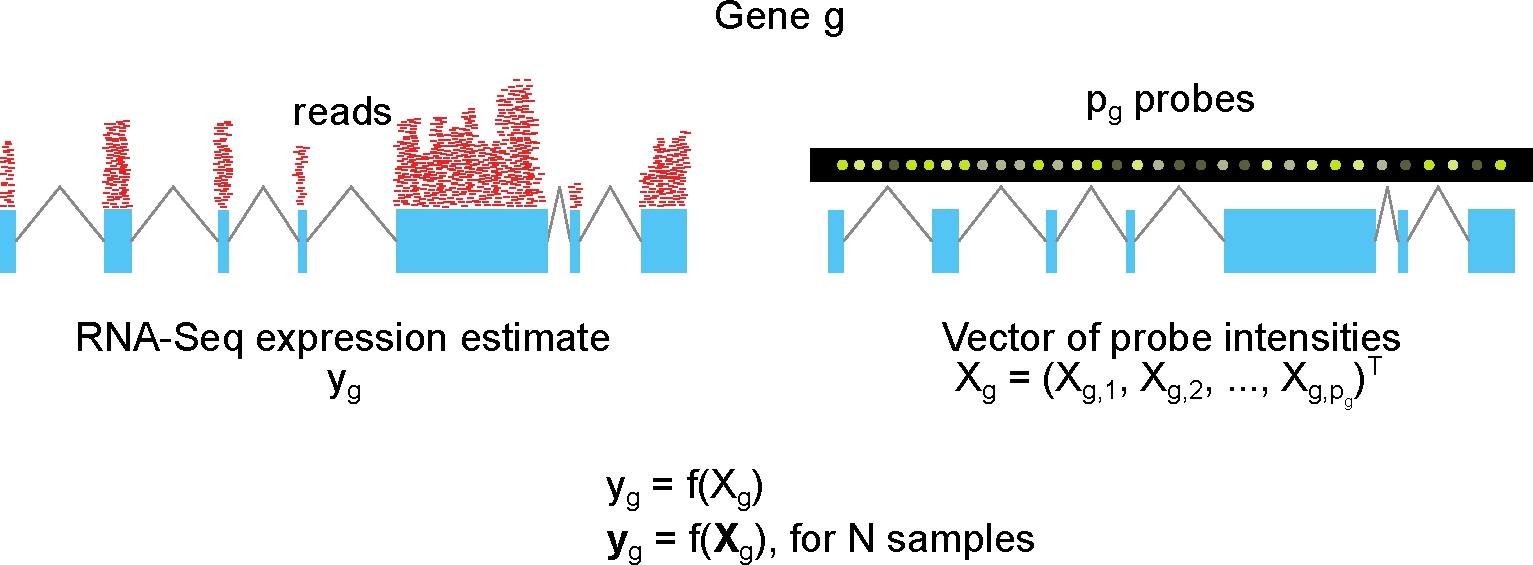
\includegraphics[width=\columnwidth]{schematic.pdf}
\caption{\textbf{Schematic of the MaLTE framework.} A supervised learning algorithm is used to learn the relationship between a gold-standard (RNA-Seq) and probe fluorescence intensities. The learned model may then be applied to a new set of probes.}
\label{fig:schematic}
\end{figure}

This approach overcomes the two main setbacks of conventional algorithms: it transforms expression estimates onto an absolute scale thus improving the within-sample correlations and naturally extends to predicting expression of individual transcript isoforms by training on the multiple responses of individual transcript isoforms. Moreover, \textsf{MaLTE} leads to substantial improvements in cross-sample correlations when used on data from the same batch, which increases statistical power. Finally, a tree-based learning introduces an easy way to filter out poorly-predicted genes through the use of out-of-bag estimates.

This documents describes how to use the \textsf{R} \textsf{MaLTE} package. It begins with a description on how to get and install the package. It then outlines the two main ways in which the package may be used: \textit{gene expression prediction (GEP)} and \textit{transcript isoform expression prediction (TIEP)}. It concludes with a description on how to filter and collate expression predictions for downstream analyses. It also provides a tentative road map for future development, a detailed description on how the \textsf{MaLTE} package is built, and includes a detailed use case of using data from the Genotype-Tissue Expression (GTEx) project \cite{lonsdale2013genotype} as training data together with an example of array transformation (e.g. from exon array to gene array). Bug reports, comments and suggestions are welcome through \href{mailto:paul.korir@gmail.com}{paul.korir@gmail.com}.

\section{Conventions Used}
\label{conventions}
\begin{itemize}
\item Array data used here corresponds to that from \textit{Affymetrix GeneChip$^{\text{\textregistered}}$ Human Exon 1.0 ST} arrays. At present only Affymetrix GeneChip$^{\text{\textregistered}}$ Human Exon and Human Gene arrays have been tested using \textsf{MaLTE}.
\item All gene and transcript identifiers are from Ensembl (\url{http://www.ensembl.org}).
\item All filenames are written in italics (\textit{filename.txt}), variables in monospace (\texttt{my.var}), and functions in monospace terminated with parentheses (\texttt{my.function()}). Classes are in monospace beginning with a capital letter (\texttt{My.Class}) while corresponding constructors additionally terminate with parentheses (\texttt{My.Class()}). Names of software packages are in sans (\textsf{R}, \textsf{MaLTE}, \textsf{Cufflinks})
\item \textit{High-throughput sequencing (HTS)} refers to \textit{RNA-Seq}.
\item A \textit{map} is a tab-delimited text file with two columns with each column consisting of identifiers/names.
\item The set of samples used for training are called \textit{training samples}. \textit{Test samples} refer to the samples that need to have their gene/transcript expression quantified.
\end{itemize}

\section{System Requirements}
\label{system}
\begin{itemize}
\item \textsf{R} (\texttt{2.14.0} or greater) installed on GNU/Linux: \textsf{MaLTE} has been tested on Scientific Linux version 5, Ubuntu 12.04, and Mac OS X.
\item  \textsf{R} packages: \texttt{party}, \texttt{multicore}, \texttt{quantrefForest}, \texttt{limma}
\item \textsf{Python} 2.7
\item Affymetrix Power Tools (APT; \url{http://www.affymetrix.com})
\item Affymetrix GeneChip® library files (\url{http://www.affymetrix.com})
\item \textsf{git} (optional)

\end{itemize}

\section{Installation}
\label{installation}
\textsf{MaLTE} may be downloaded from \url{https://github.com/polarise/MaLTE-package}. There are two ways to install \textsf{MaLTE}: via GNU/Linux shell and \textsf{R} shell.

\begin{enumerate}
\item Via GNU/Linux shell
\begin{verbatim}
R CMD INSTALL MaLTE_<release>.tar.gz
\end{verbatim}

\item Via \textsf{R} shell
\begin{verbatim}
> install.packages( "/path/to/MaLTE_<release>.tar.gz" )
\end{verbatim}
\end{enumerate}

\noindent\\
Once installed, \textsf{MaLTE} should be loaded in the \textsf{R} shell as follows:
\begin{verbatim}
> library( MaLTE )
\end{verbatim}
or, quietly
\begin{verbatim}
> suppressMessages( library( MaLTE ))
\end{verbatim}

\section{Example Dataset}
\label{datasets}
Example data files are provided with \textsf{MaLTE}, which are based on data from the HapMap project \cite{gibbs2003international}. These are all contained in the \texttt{data} directory in the package. They will be used in Section~\ref{gep} and Section~\ref{tiep} and are formatted as outlined in Section~\ref{gep:detailed} and Section~\ref{tiep:detailed}.

\begin{enumerate}
\item Files with sample names (several examples provided)
\item HTS data
\item Transcript HTS data
\item Raw microarray data (direct output from APT \texttt{apt-cel-extract})
\item Truncated microarray data (non-essential rows and columns removed)
\item Gene-to-probeset maps for exon array
\item Gene-to-transcript maps
\end{enumerate}

The complete set of files may be displayed on the \textsf{R} shell using the following line:
\begin{verbatim}
> dir( paste( system.file( package="MaLTE" ), "data", sep="/" ))
\end{verbatim} 

\section{Gene Expression Prediction}
\label{gep}
\subsection{Quick Start Guide}
\label{gep:quick}
This section provides a quick introduction to using \textsf{MaLTE}. Detailed instructions incorporating descriptions of the various file and there respective formats is provided in Section \ref{gep:detailed}. It is assumed that the user is in the \textsf{R} shell, the \textsf{MaLTE} library is loaded and the following data files are available: \textit{samples.txt}, \textit{hts\_data.txt}, \textit{ma\_data.txt}, \textit{gene\_probesets.txt}.

\noindent\\
\textbf{Step I:} Provide the location of the file containing a map between sample names on both platforms (RNA-Seq and microarray)
\begin{verbatim}
> samples.fn = paste( system.file( package="MaLTE" ), "data", 
  "samples.txt.gz", sep="/" )
\end{verbatim}

\noindent\\
\textbf{Step II:} Provide the location of the file containing the high-throughput sequencing (RNA-Seq) data
\begin{verbatim}
> hts.fn = paste( system.file( package="MaLTE" ), "data", 
  "hts_data.txt.gz", sep="/" )
\end{verbatim}

\noindent\\
\textbf{Step III:} Provide the location to the file containing quantile-normalized and background corrected fluorescence probe intensities
\begin{verbatim}
> ma.fn = paste( system.file( package="MaLTE" ), "data", 
  "ma_data.txt.gz", sep="/" )
\end{verbatim}

\noindent\\
\textbf{Step IV:} Provide the location of a map showing the probe sets associated with each gene
\begin{verbatim}
> g2p.fn = paste( system.file( package="MaLTE" ), "data", 
  "gene_probesets.txt.gz", sep="/" )
\end{verbatim}

\noindent\\
\textbf{Step V:} Prepare the data into training and test sets
\begin{verbatim}
> prepare.data( samples.fn=samples.fn, ma.fn=ma.fn, hts.fn=hts.fn, 
  g2p.fn=g2p.fn )
\end{verbatim}

\noindent\\
\textbf{Step VI:} Read the data in preparation for the training and test phase
\begin{verbatim}
> tt.ready = read.data( train.fn="train_data.txt.gz", 
  test.fn="test_data.txt.gz" )
\end{verbatim}

\noindent\\
\textbf{Step VII:} Initialize training parameters
\begin{verbatim}
# conditional random forest
> tt.params = TT.Params()

# quantile regression random forest
> tt.params = TT.Params( quantreg=TRUE )
\end{verbatim}

\noindent\\
\textbf{Step VIII:} Train and predict
\begin{verbatim}
> tt.seq = array2seq( tt.ready, tt.params )
\end{verbatim}

\noindent\\
\textbf{Step IX:} Perform out-of-bag (OOB) predictions
\begin{verbatim}
> tt.seq.oob = array2seq.oob( tt.ready, tt.params )
\end{verbatim}

\noindent\\
\textbf{Step X:} Filter based on OOB correlations
\begin{verbatim}
> tt.filtered = oob.filter( tt.seq, tt.seq.oob, thresh=0 )
\end{verbatim}

\noindent\\
\textbf{Step XI:} Get the names of test samples
\begin{verbatim}
> test.names = get.names( samples.fn, test=TRUE )
\end{verbatim}
or 
\begin{verbatim}
> test.names = get.test( samples.fn )   # get test sample names
\end{verbatim}

\noindent\\
\textbf{Step XII:} Aggregate predictions and write output to a text file for downstream analyses.
\begin{verbatim}
> df = get.predictions( tt.filtered, test.names )
> write.table( df, file="filt_preds.txt", col.names=TRUE, row.names=FALSE, 
  quote=FALSE, sep="\t" )
\end{verbatim}

\subsection{Detailed Instructions}
\label{gep:detailed}
Gene expression prediction (GEP) depends on having four input files:
\begin{itemize}
\item \textbf{Sample names.} A map of sample names between both platforms (HTS and array; possibly zipped). An example file is provided with the package (Step I).
\item \textbf{HTS data.} The HTS (RNA-Seq) data in text file (possibly zipped)
\item \textbf{Microarray data.} The microarray probe data (possibly zipped) 
\item \textbf{Gene-to-probeset map.} A map between gene identifiers and probe set identifiers. Probe set identifiers are provided by the array manufacturer as part of the array description.
\end{itemize}

Each file is now described in detail under the following sub-headings: \textit{purpose}, \textit{generic designation}, \textit{header} and \textit{structure}.

\subsubsection{Sample Names File}
\label{gep:sample}

\begin{tabular}{rp{12cm}}
\textbf{Purpose} & This file provides a one-to-one map between sample identifiers on both platforms. \\
\textbf{Generic designation} & \textit{samples.txt} OR \textit{samples.txt.gz}; Any suitable name will do but the file name must end either with \textit{*.txt} or \textit{*.txt.gz}. \\
\textbf{Header} & \texttt{hts\textless tab\textgreater ma} \\
\textbf{Structure} & Two-columns separated by a single tab (tab-delimited) \\
  & All sample identifiers must be unique and must exactly correspond to sample names present in the headers of the HTS data and microarray data (to be described shortly). For example, microarray probe files will usually have headers with sample names terminated by \textit{*.CEL}; this must be retained in the sample names file. \\
  & Test samples are marked by having an asterisk (\texttt{`*'}) as the first character. Any other row is assumed to be a training sample. \\
  & Test samples may consist of having both HTS and array data. If only test array data is present then the first column must be \texttt{`*NA'}. \\
  & Comments must begin with a pound/hash (\texttt{`\#'}) symbol. \\
\end{tabular}

\subsubsection{HTS Data File}
\label{gep:hts}

\begin{tabular}{rp{12cm}}
\textbf{Purpose} & This file provides the HTS expression estimates.\\
\textbf{Generic designation} & \textit{hts\_data.txt} OR \textit{hts\_data.txt.gz} \\
  & Any suitable name will do but the file name must end either with \textit{*.txt} or \textit{*.txt.gz}. \\
\textbf{Header} & \texttt{gene\_id\textless tab\textgreater Sample01\textless tab\textgreater...\textless tab\textgreater SampleN} \\
\textbf{Structure} & Tab-delimited \\
  & All rows must be unique \\
  & No comments are allowed \\
\end{tabular}

\subsubsection{Microarray Data File}
\label{gep:microarray}

\begin{tabular}{rp{12cm}}
\textbf{Purpose} & This file provides the microarray probe intensities. \\
\textbf{Generic designation} & \textit{ma\_data.txt} OR \textit{ma\_data.txt.gz} if inessential columns have been removed (see Section \ref{gep:prepare} on \textit{Preparing Input Files})
\textit{raw\_ma\_data.txt} OR \textit{raw\_ma\_data.txt.gz} if inessential columns are still present (see Section \ref{gep:prepare} on \textit{Preparing Input Files}) \\
  & Any suitable name will do but its name must terminate with \textit{*.txt} or \textit{*.txt.gz}. \\
\textbf{Header} & \texttt{probe\_id\textless tab\textgreater Sample01\textless tab\textgreater...\textless tab\textgreater SampleN} \\
\textbf{Structure} & Tab-delimited \\
  & Comments must begin with a pound/hash (\texttt{`\#'}) symbol. \\
\end{tabular}

\subsubsection{Gene-to-Probe Set Map}
\label{gep:gene}

\begin{tabular}{rp{12cm}}
\textbf{Purpose} & This file provides a one-to-many map of gene identifiers to probe set identifiers. \\
\textbf{Generic designation} & \textit{gene\_probesets.txt} OR \textit{gene\_probesets.txt.gz} \\
  & Any suitable name will do but the file name must end either with \textit{*.txt} or \textit{*.txt.gz}.. \\
\textbf{Header} & \texttt{gene\_id\textless tab\textgreater probeset\_id} \\
\textbf{Structure} & Tab-delimited \\
  & Probe set identifiers may be missing for some genes. \\
  & No comments are allowed. \\
\end{tabular}

\subsection{Preparing Input Files}
\label{gep:prepare}
\begin{enumerate}
\item \textbf{Sample names.} This file can be prepared using a text editor or preferably using a spreadsheet application such as Microsoft Excel or LibreOffice/OpenOffice Calc. The file must be saved as a tab-delimited text file or a comma-separated values (CSV) file with the field-delimiter set to TABS and the quote-character set to NONE. The file extension must be as described above.

\item \textbf{HTS data.} This file may be constructed using customized scripts that collate the HTS expression estimates output from programs such as \textsf{Cufflinks} or \textsf{DESeq}. The order of sample columns is unimportant. There are several online datasets\footnote{\url{http://bowtie-bio.sourceforge.net/recount/}} that are provided in this format making it easy to proceed with using \textsf{MaLTE}.

\item \textbf{Microarray data.} Raw microarray data is provided as CEL files. The contents of CEL files need to be extracted and additional pre-processing steps may be applied to the raw data. Two pre-processing steps we recommend are quantile-normalization (QN) and background correction (BC). The Affymetrix Power Tools (APT) suite is recommended for this and other analytical steps though several \textsf{R} packages have been developed to supplement APT.  Here we describe how to extract fluorescence probe intensities and how to remove unnecessary columns.

\begin{enumerate}
\item[(i)] \textbf{Extracting QN and BC microarray probe data.} We assume that all CEL files are contained in a single folder. APT requires a set of library files that are available from the Affymetrix website (\url{http://www.affymetrix.com}). An account will have to be created in order to download library files. The library files consist of array description files used by APT to carry out analyses. More information on these can be found in the manuals provided for each array type. 

To extract probes with QN and BC:
\begin{verbatim}
apt-cel-extract -o raw_ma_data.txt 
  -c /path/to/HuEx-1_0-st-v2.2/HuEx-1_0-st-v2.r2.clf 
  -p /path/to/HuEx-1_0-st-v2.2/HuEx-1_0-st-v2.r2.pgf 
  -b /path/to/HuEx-1_0-st-v2.2/HuEx-1_0-st-v2.r2.antigenomic.bgp 
  -a quant-norm,pm-gcbg *.CEL
\end{verbatim}

This provides `raw' data that can directly be used with \textsf{MaLTE}. To do so, the \texttt{raw} argument in \texttt{prepare.data()} must be set to \texttt{TRUE} (as it is \texttt{FALSE} by default). However, unnecessary columns can be excluded as shown below.

\item[(ii)] \textbf{Excluding unnecessary columns.} Unnecessary columns can be easily excluded using the bash utility \texttt{cut} as follows:

\begin{verbatim}
cut -f1,5,8- raw_ma_data.txt > ma_data.txt
\end{verbatim}

\end{enumerate}

\item \textbf{Zip the file to save space.}
\begin{verbatim}
gzip raw_ma_data.txt
gzip ma_data.txt
\end{verbatim}

\item \textbf{Gene-to-probeset map.} This file may be downloaded directly from \textsf{BioMart}, particularly for popular arrays. Alternatively, the user may prepare it for him/herself. This can be done using \textsf{BEDTools}. \textsf{BEDTools} takes as input two BED files having coordinates of gene and probe sets, respectively. The \texttt{intersect} \textsf{BEDTools} utility then finds all overlaps between both files and writes them to an extended BED file. The appropriate columns can then be combined to provide the required file.

To use the BED approach, the gene annotation must be provided as a BED file. Similarly, the array's annotation files (available from the Affymetrix website) must be converted to BED format. Both tasks may be performed using custom scripts.

Please consult the \textsf{BEDTools} website (\url{http://bedtools.readthedocs.org/en/latest/}) on how to intersect two BED files.

The gene and probe set columns can then be isolated using \texttt{cut} in a manner similar to sub-step (2) above.
\end{enumerate}


\section{Transcript Isoform Expression Prediction}
\label{tiep}

\subsection{Quick Start Guide}
\label{tiep:quick}
This section describes how to perform transcript isoform expression prediction in quick steps. It assumes that the user has logged into an \textsf{R} shell, the \textsf{MaLTE} package is loaded and that the following files are available: \textit{samples.txt}, \textit{train\_data.txt.gz}, \textit{test\_data.txt.gz}, \textit{hts\_txs\_data.txt}, and \textit{gene\_transcripts.txt}.

The files \textit{train\_data.txt.gz} and \textit{test\_data.txt.gz} are produced by running Step I-V in Section \ref{gep:quick} \textit{Gene Expression Prediction: Quick Start Guide}.

\noindent\\
\textbf{Step I:} Provide the location of the file containing a map between sample names on both platforms (RNA-Seq and microarray)
\begin{verbatim}
> samples.fn = paste( system.file( package="MaLTE" ), "data", 
  "samples.txt.gz", sep="/" )
\end{verbatim}

\noindent\\
\textbf{Step II:} Provide the location of the file containing the high-throughput sequencing (RNA-Seq) transcript isoform expression estimates
\begin{verbatim}
> hts.txs.fn = paste( system.file( package="MaLTE" ), "data", 
  "hts_txs_data.txt.gz", sep="/" )
\end{verbatim}

\noindent\\
\textbf{Step III:} Provide the location of map of gene-to-transcript identifiers
\begin{verbatim}
> g2tx.fn = paste( system.file( package="MaLTE" ), "data", 
  "gene_transcripts.txt.gz", sep="/" )
\end{verbatim}

\noindent\\
\textbf{Step IV:} Prepare the data into training and test sets
\begin{verbatim}
> prepare.txs.data( samples.fn=samples.fn, train.fn="train_data.txt.gz", 
  test.fn="test_data.txt.gz", hts.txs.fn=hts.txs.fn, g2tx.fn=g2tx.fn )
\end{verbatim}

\noindent\\
\textbf{Step V:} Read in the data in preparation for training and preparation
\begin{verbatim}
> tt.ready.txs = read.txs.data( train.fn="train_txs_data.txt.gz", 
  test.fn="test_txs_data.txt.gz" )
\end{verbatim}
\textbf{Step VI:} Train and predict
\begin{verbatim}
> tt.seq.txs = array2seq( tt.ready.txs, tt.params )
\end{verbatim}

\noindent\\
\textbf{Step VII:} Train and predict for OOB estimates
\begin{verbatim}
> tt.seq.oob.txs = array2seq.oob( tt.ready.txs, tt.params )
\end{verbatim}
\textbf{Step VIII:} Filter based on OOB correlations
\begin{verbatim}
> tt.filtered.txs = oob.filter( tt.seq.txs, tt.seq.oob.txs, thresh=0 )
\end{verbatim}

\noindent\\
\textbf{Step IX:} Get test sample names
\begin{verbatim}
> test.names = get.names( samples.fn, test=TRUE )
\end{verbatim}
or 
\begin{verbatim}
> test.names = get.test( samples.fn )   # get test sample names
\end{verbatim}

\noindent\\
\textbf{Step X:} Collate predicted transcript isoform predictions and write them to a text file for downstream analyses
\begin{verbatim}
> df.txs = get.predictions( tt.filtered.txs, test.names )
\end{verbatim}

\subsection{Detailed Instructions}
\label{tiep:detailed}
Transcript isoform expression prediciton (TIEP) depends on having five input files:
\begin{itemize}
\item \textbf{Sample names.} A map of sample names between both platforms (HTS and array; possibly zipped). This is the exact same file used in GEP above.
\item \textbf{GEP Training data.} The name of this file is \textit{train\_data.txt.gz}. It is the first zipped output produced by running \texttt{prepare.data()} prior to carrying out GEP.
\item \textbf{GEP Test data.} The name of this file is \textit{test\_data.txt.gz}. It is the second zipped output produced by running \texttt{prepare.data()} prior to carrying out GEP.
\item \textbf{Transcript HTS data.} The HTS (RNA-Seq) transcript isoform data in text file (possibly zipped)
\item \textbf{Gene-to-transcript map.} A map of between gene identifiers and transcript identifiers. 
\end{itemize}

\subsubsection{Sample Names File}
\label{tiep:sample}

\begin{tabular}{rp{12cm}}
\textbf{Purpose} & This file provides a one-to-one map between sample identifiers on both platforms. \\
\textbf{Generic designation} & \textit{samples.txt} OR \textit{samples.txt.gz} \\
   & Any suitable name will do but the file name must end either with \textit{*.txt} or \textit{*.txt.gz}.. \\
\textbf{Header} & \texttt{hts\textless tab\textgreater ma} \\
\textbf{Structure} & Two-columns separated by a single tab (tab-delimited) \\
  & All sample identifiers must be unique and must exactly correspond to sample names present in the headers of the HTS data and microarray data. For example, microarray probe files will usually have headers with sample names terminated by \textit{*.CEL}; this must be retained in the sample names file. \\
  & Test samples are marked by having an asterisk (\texttt{`*'}) as the first character. Any other row is assumed to be a training sample. \\
  & Test samples may consist of having both HTS and array data. If only test array data is present then the first column must be \texttt{`*NA'}. \\
  & Comments must begin with a pound/hash (\texttt{`\#'}) symbol. \\
\end{tabular}

\subsubsection{GEP Training Data File}
\label{tiep:gep_train}

\begin{tabular}{rp{12cm}}
\textbf{Purpose} & This file contains gene-to-probe training data that will be used to create new transcripts-to-probes training data. \\
\textbf{Generic designation} & \textit{train\_data.txt.gz} \\
  & This file is produced after running \texttt{prepare.data()}. \\
\textbf{Header} & None \\
\textbf{Structure} & This file has six columns. This data is automatically generate by the \texttt{prepare.data()} function. \\
  & Gene identifier \\
  & Number of training samples \\
  & Number of probes associated with this gene \\
  & Probe (not probe set) identifiers associated with this gene \\
  & HTS expression estimates \\
  & Vectorized matrix\footnotemark[1] of fluorescence probe intensities \\
\end{tabular}
\footnotemark[1]{A \textit{vectorized matrix} is a stack of the columns into a single column vector.}

\subsubsection{GEP Test Data File}
\label{tiep:gep_test}

\begin{tabular}{rp{12cm}}
\textbf{Purpose} & This file contains that gene-to-probe training data that will be used to create new transcripts-to-probes training data. \\
\textbf{Generic designation} & \textit{test\_data.txt.gz} \\
\textbf{Header} & None \\
\textbf{Structure} & This file has six columns. This data is automatically generate by the \texttt{prepare.data()} function. \\
  & Gene identifier \\
  & Number of test samples \\
  & Number of probes associated with this gene \\
  & Probe (not probe set) identifiers associated with this gene \\
  & HTS expression estimates \\
  & Vectorized matrix of fluorescence probe intensities
\end{tabular}

\subsubsection{Transcript HTS Data File}
\label{tiep:transcript}

\begin{tabular}{rp{12cm}}
\textbf{Purpose} & This file provides the HTS transcript isoform expression estimates. \\
\textbf{Generic designation} & \textit{hts\_txs\_data.txt} OR \textit{hts\_txs\_data.txt.gz} \\
  & Any suitable name will do but the file name must end either with \textit{*.txt} or \textit{*.txt.gz}.. \\
\textbf{Header} & \texttt{tx\_id\textless tab\textgreater Sample01\textless tab\textgreater...\textless tab\textgreater SampleN} \\
\textbf{Structure} & Tab-delimited \\
  & All rows must be unique \\
  & No comments are allowed \\
\end{tabular}

\subsubsection{Gene-to-Transcript Map}
\label{tiep:gene}

\begin{tabular}{rp{12cm}}
\textbf{Purpose} & This file provides a one-to-many map of gene identifiers to transcript  identifiers. \\
\textbf{Generic designation} & \textit{gene\_transcripts.txt} OR \textit{gene\_transcripts.txt.gz} \\
  & Any suitable name will do but the file name must end either with \textit{*.txt} or \textit{*.txt.gz}.. \\
\textbf{Header} & \texttt{gene\_id\textless tab\textgreater tx\_id} \\
\textbf{Structure} & Tab-delimited \\
  & No comments are allowed. \\
\end{tabular}

\subsection{Preparing Input Files}
\label{tiep:prepare}
\begin{enumerate}
\item \textbf{Sample names.} Please see Section~\ref{gep} \textit{GEP: Preparing Input Files}.

\item \textbf{GEP training data.} This file is automatically generated after running \texttt{prepare.data()} Please see Section~\ref{gep} Steps I-V of \textit{GEP: Quick Start Guide}.

\item \textbf{GEP test data.} This file is automatically generated after running \texttt{prepare.data()} Please see Section~\ref{gep} Steps I-V of \textit{GEP: Quick Start Guide}.

\item \textbf{Transcript HTS data file.} Several programs are available that perform transcript isoform expression quantification from HTS data. Widely used examples include \textsf{Cufflinks}, \textsf{IsoEM} and \textsf{RSEM}. As suggested in HTS data description in Section \ref{gep:prepare} \textit{GEP: Preparing Input Files}, custom scripts should be used to combine expression estimates. Sample names in the header must exactly correspond to those in the Sample names file. The order of samples is not important.

\item \textbf{Gene-to-transcript map.} A man of gene to transcript identifiers is most easily obtained from \textsf{BioMart}.
\end{enumerate}

\section{Filtering and Collating Predictions}
\label{filtering}

The training and prediction step produces data in an internal format that is not suitable for further bioinformatic analyses. The prediction estimates need to be filtered to exclude poor predictions then finally converted into a data frame that can then be saved as a tab-delimited text file. Steps IX and X show GEP OOB filtering and step VII and VIII show TIEP OOB filtering. In order for expression predictions to be collated, the sample names must first be obtained (GEP: Step XI; TIEP: Step X) from the sample names file (\textit{samples.txt}). Finally, extracted data may be written to a tab-delimited text file using base \textsf{R} functions.

Filtering takes advantage of the tree-based learning algorithm. Conditional random forests are used in the current implementation of \textsf{MaLTE}. A forest is an ensemble of trees, with each tree constructed by bootstrapping on the training data then using a recursive partition approach to define the branches. The forest consists of hundreds to thousands of such trees and predictions are aggregated either by a simple voting scheme (classification) or averaging (regression). Each training observation is used to train a subset of all the trees therefore the trees from which it is absent (for which it is \textit{out-of-bag}) can be used to predict its value. The resulting predicted estimates are therefore called the \textit{out-of-bag (OOB) estimates} from which we can estimate a correlation with the training response. It is this correlation that acts as a heuristic for prediction performance and results in \textit{OOB filtering}. An OOB Pearson correlation threshold of zero ($r_{\mathrm{OOB}} > 0$) is currently set as a default filter threshold.

Alternatively, filtering can be based on the training RPKM/FPKM values. For example, we could include all genes with at least ten samples with an FPKM above one.

\begin{verbatim}
# tt.seq     - predictions from training data 
# tt.seq.oob - OOB predictions (contains training RNA-Seq)
# only include genes with at least 10 samples having
#  RNA-Seq expression of at least 1
> filt.indexes = .filter.trues( tt.seq.oob, filter.fpkm=1, filter.count=10 )
> tt.filt = tt.seq[ filt.indexes ]

# extract a data frame of filtered predictions
> test.names = get.test( samples.fn ) # get names of test samples
> df.malte = get.predictions( tt.filt, test.names )
\end{verbatim}

\section{Training Parameters}
\label{params}

There are eight main parameters that can be specified when running \textsf{MaLTE:}

\begin{verbatim}
> tt.params = TT.Params()
> tt.params
mtry             = 2 
ntree            = 1000 
feature.select   = TRUE 
min.probes       = 15 
cor.thresh       = 0 
OOB              = FALSE 
QuantReg         = FALSE 
Tune (OOB cor.P) = NA
\end{verbatim} 

\begin{enumerate}
\item \textbf{\texttt{mtry.}} Specifies the number of predictors (probes) to be used in creating splits in the tree. The default and optimized parameter value is \texttt{mtry=2}.
\item \textbf{\texttt{ntree.}} The number of trees in the forest. The default and optimized value is \texttt{ntree=1000}.
\item \textbf{\texttt{feature.select.}} A boolean that sets whether feature selection is carried out. The default value is \texttt{feature.select=TRUE}.
\item \textbf{\texttt{min.probes.}} If \texttt{feature.select=TRUE} then what is the minimum number of probes below which no feature selection is carried out? Defaults to \texttt{min.probes=15} (i.e. feature selection is only carried out for 16 or more probes).
\item \textbf{\texttt{cor.thresh.}} Feature selection is implemented using a simple method: the top \texttt{min.probes} probes that correlate with the response (RNA-Seq) are used if they have a Pearson correlation of at least \texttt{cor.thresh}.
\item \textbf{\texttt{OOB.}} A boolean that specifies whether or not OOB predictions are performed. Defaults to \texttt{OOB=FALSE}.
\item \textbf{\texttt{quantreg.}} A boolean that specifies whether or not to use quantile regression forest as the learner. Defaults to \texttt{quantreg=FALSE}.
\item \textbf{\texttt{tune.}} This is an experimental feature in which parameter values are tune for each gene individually. Parameters are tuned in a cascade in the following order: \texttt{feature.select}, \texttt{mtry}, then \texttt{ntree}. Other parameters are retained as specified above. Defaults to \texttt{tune=FALSE}.
\end{enumerate}

\section{Future Work}
\label{future}
The following list of features may be added at a future date:
\begin{enumerate}
\item \textbf{Replace the underlying \textsf{Python} scripts with C/C++ programs.} We used \textsf{Python} because it was relatively simple to put together and it has mature data structures. \textsf{Python} scripts are slower than \textsf{C/C}\verb!++! programs but we have applied multiprocessing to shorten the data preparation step. However, this arrangement restricts \textsf{MaLTE} to UNIX-like systems.
\item \textbf{Configure training and test data using a standardised structured file format.} Currently, training and test data is held in custom tab-delimited files. We would like to transition either to XML or HDF.
\item \textbf{Expand the use of the sample names (\textit{samples.txt}) file.} Currently, the sample names file is underutilised. It is possible to include additional columns that could be incorporated into the learning process. For example, a column on batch information could be passed to \textsf{ComBat} to minimise batch effects. Other variables such as tissue type could be important for training.
\item \textbf{Automatic parameter tuning.} We would like to incorporate a tuning utility that uses a random sample of the training data to optimise the training parameters.
\end{enumerate}

\section{Bug Reports}
\label{bugs}
Please send bug reports and feature requests to \href{mailto:paul.korir@gmail.com}{paul.korir@gmail.com} with the subject `MaLTE Bugs' of `MaLTE Features', respectively. Alternatively, you may visit \url{https://github.com/polarise/MaLTE/issues} and click the `Issues' button to file a report.

\section{Citing \textsf{MaLTE}}
\textsf{MaLTE} has been submitted for peer-review. This section will be updated shortly.

\begin{thebibliography}{50}

\bibitem{irizarry2003summaries} Irizarry, Rafael A., et al. "Summaries of Affymetrix GeneChip probe level data." Nucleic acids research 31.4 (2003): e15-e15.
\bibitem{irizarry2005multiple} Irizarry, Rafael A., et al. "Multiple-laboratory comparison of microarray platforms." Nature Methods 2.5 (2005): 345-350.
\bibitem{fu2009estimating} Fu, Xing, et al. "Estimating accuracy of RNA-Seq and microarrays with proteomics." BMC Genomics 10.1 (2009): 161.
\bibitem{irizarry2006comparison} Irizarry, Rafael A., Zhijin Wu, and Harris A. Jaffee. "Comparison of Affymetrix GeneChip expression measures." Bioinformatics 22.7 (2006): 789-794.
\bibitem{lonsdale2013genotype}
John Lonsdale, Jeffrey Thomas, Mike Salvatore, Rebecca Phillips, Edmund Lo,
  Saboor Shad, Richard Hasz, Gary Walters, Fernando Garcia, Nancy Young, et~al.
\newblock {The Genotype-Tissue Expression (GTEx) project}.
\newblock {\em Nature Genetics}, 45(6):580--585, 2013.
\bibitem{malone2011microarrays} Malone, John H., and Brian Oliver. "Microarrays, deep sequencing and the true measure of the transcriptome." BMC biology 9.1 (2011): 34.
\bibitem{gibbs2003international} Gibbs, Richard A., et al. "The international HapMap project." Nature 426.6968 (2003): 789-796.

\end{thebibliography}

\pagebreak
\appendix
\section{Classes}
\label{classes}
The \textsf{R} \textsf{MaLTE} package uses three main classes.
\begin{enumerate}
\item \texttt{TT.Ready}. This class handles data \textit{ready} for training and test. It is an abstract base class from which two other classes are derived:
\begin{enumerate}
\item[(i)] \texttt{TT.Ready.Gene}. This class handles gene expression training and prediction data.
\item[(ii)] \texttt{TT.Ready.Txs}. This is for transcript isoform expression data.
\end{enumerate}

\item \texttt{TT.Seq}. This class handles the results of training and prediction. Just like \texttt{TT.Ready}, this is an abstract base class with two derived classes:
\begin{enumerate}
\item[(i)] \texttt{TT.Seq.Gene} for gene predictions. Both test and OOB predictions are of this class.
\item[(ii)] \texttt{TT.Seq.Txs} for transcript isoform predictions similar to \texttt{TT.Seq.Gene}.
\end{enumerate}

\item \texttt{TT.Params}. This class handles training and prediction parameters passed to the \texttt{train.and.predict()} (alias \texttt{run()}) methods of \texttt{TT.Ready} objects. It has the following slots: \texttt{mtry}, \texttt{ntree}, \texttt{feature.select}, \texttt{min.probes}, \texttt{cor.thresh}, \texttt{OOB}, \texttt{quantreg}, \texttt{tune}.
\end{enumerate}

More information on these classes can be found in the \textsf{MaLTE} manual that accompanies the package.

\pagebreak
\begin{landscape}
\section{Function and Methods Table}
\label{functions}

\begin{table}[H]
\scriptsize
\centering
\begin{tabular}{|p{2.5cm}|p{6cm}|p{4cm}|p{5cm}|}
\hline
\textbf{Function/Method} & \textbf{Input} & \textbf{Output} & \textbf{Comments} \\
\hline
\texttt{prepare.data()} & \texttt{samples.fn}, \texttt{ma.fn} (OR \texttt{raw\_ma.fn} with \texttt{raw=TRUE}), \texttt{hts.fn}, \texttt{g2p.fn} & \textit{train\_data.txt.gz} and \textit{test\_data.txt.gz}  (together with log files indicating which genes are missing) & This function calls the underlying \textsf{Python} script \textit{prepare\_data.py}, which can be called directly by the user. All output is written to the current directory. \\
\hline
\texttt{read.data()} & \texttt{train.fn=`train\_data.txt.gz'}, \texttt{test.fn=`test\_data.txt.gz'} & \texttt{tt.ready} & \texttt{tt.ready} is a list of objects of class \texttt{TT.Ready.Gene} that has embedded within it the training and testing data. \\
\hline
\texttt{prepare.txs.data()} & \texttt{samples.fn}, \texttt{train.fn}, \texttt{test.fn}, \texttt{hts.txs.fn}, \texttt{g2tx.fn} & \textit{train\_txs\_data.txt.gz}, \textit{test\_txs\_data.txt.gz} (together with log files indicating which genes are missing) & 
This function works like \texttt{prepare.data()} by calling the undlying \textsf{Python} script \textit{prepare\_txs\_data.py}, which can be called directly. All output is written to the current directory. \\
\hline
\texttt{read.txs.data()} & \texttt{train.fn=`train\_txs\_data.txt.gz'}, \texttt{test.fn=`test\_txs\_data.txt.gz'} & \texttt{tt.ready.txs} & \texttt{tt.ready.txs} is a list of objects of class \texttt{TT.Ready.Txs} \\
\hline
\texttt{TT.Params()} & \texttt{mtry=2}, \texttt{ntree=1000}, \texttt{feature.select=TRUE}, \texttt{min.probes=15}, \texttt{cor.thresh=0}, \texttt{OOB=FALSE}, \texttt{quantreg=FALSE}, \texttt{tune=FALSE} & \texttt{tt.params} & Constructor for objects of class \texttt{TT.Params} \\
\hline
\texttt{run()}, \texttt{oob.run()} & \texttt{TT.Ready} object, \texttt{tt.params}, \texttt{OOB=FALSE} & \texttt{TT.Seq} object & Performs prediction on a single \texttt{TT.Ready.Gene} or \texttt{TT.Ready.Txs} object. \\
\hline
\texttt{array2seq()}, \texttt{array2seq.oob()} & \texttt{tt.ready}/\texttt{tt.ready.txs}, \texttt{tt.params} & \texttt{tt.seq} OR \texttt{tt.seq.txs} & \texttt{tt.seq} is a list of \texttt{TT.Seq.Gene} or \texttt{TT.Seq.Tx} objects. \\
 & & & The parallelised-list version of \texttt{run()/oob.run()} \\
%  & & & The tuned parameters are obtained by running 'tune'. \\
\hline
\texttt{oob.filter()} & \texttt{tt.seq/tt.seq.txs}, \texttt{tt.seq.oob/tt.seq.oob.txs} (resp.), \texttt{thresh} & \texttt{tt.filtered} & \texttt{tt.filtered} is a list of objects of class \texttt{TT.Seq.Gene} \\
 & & & \texttt{tt.filtered.txs} is a list of objects of class \texttt{TT.Seq.Tx} \\
\hline
% *\texttt{tune()} & \texttt{tt.ready} & \texttt{tt.params} & Uses the training data to find the best parameters to use. Evaluation is based on OOB estimates only. \\
%  & & & \texttt{tt.params} is an object of class \texttt{TT.Params} \\
% \hline
\texttt{predictions()} & \texttt{TT.Seq.Gene} OR \texttt{TT.Seq.Txs} & \texttt{tt.predicted} OR \texttt{tt.predicted.txs} & Method to extract predictions only \\
\hline
\texttt{get.predictions()} & \texttt{tt.filtered} OR \texttt{tt.filtered.txs} & \texttt{df} & \texttt{df} is a data frame of predictions \\
\hline
\texttt{cor.P()} & \texttt{tt.seq.oob} OR \texttt{tt.seq.oob.txs} &  & Method to extract Pearson correlations only when HTS is available for test data \\
\hline
\texttt{cor.S()} & \texttt{tt.seq.oob} OR \texttt{tt.seq.oob.txs} &  & Method to extract Spearman correlations only when HTS is available for test data \\
\hline
\texttt{get.names()}, \texttt{get.train()}, \texttt{get.test()} & \texttt{samples.fn=`samples.txt'} & \texttt{sample.names} & Returns a list of names of train/test samples \\
\hline
\end{tabular}
\end{table}
\end{landscape}

\pagebreak
\section{Use Case: MaLTE Trained with GTEx Data Applied on Exon Array}
\label{usecase}

Using \textsf{MaLTE} with the GTEx training dataset consists of three main steps illustrated in Figure \ref{fig:usecase}.

\begin{itemize}
\item Obtaining the package and training data
\item Preparing the data for training-and-testing
\item Predicting, filtering and collating expression estimates
\end{itemize}

\begin{figure}
\centering
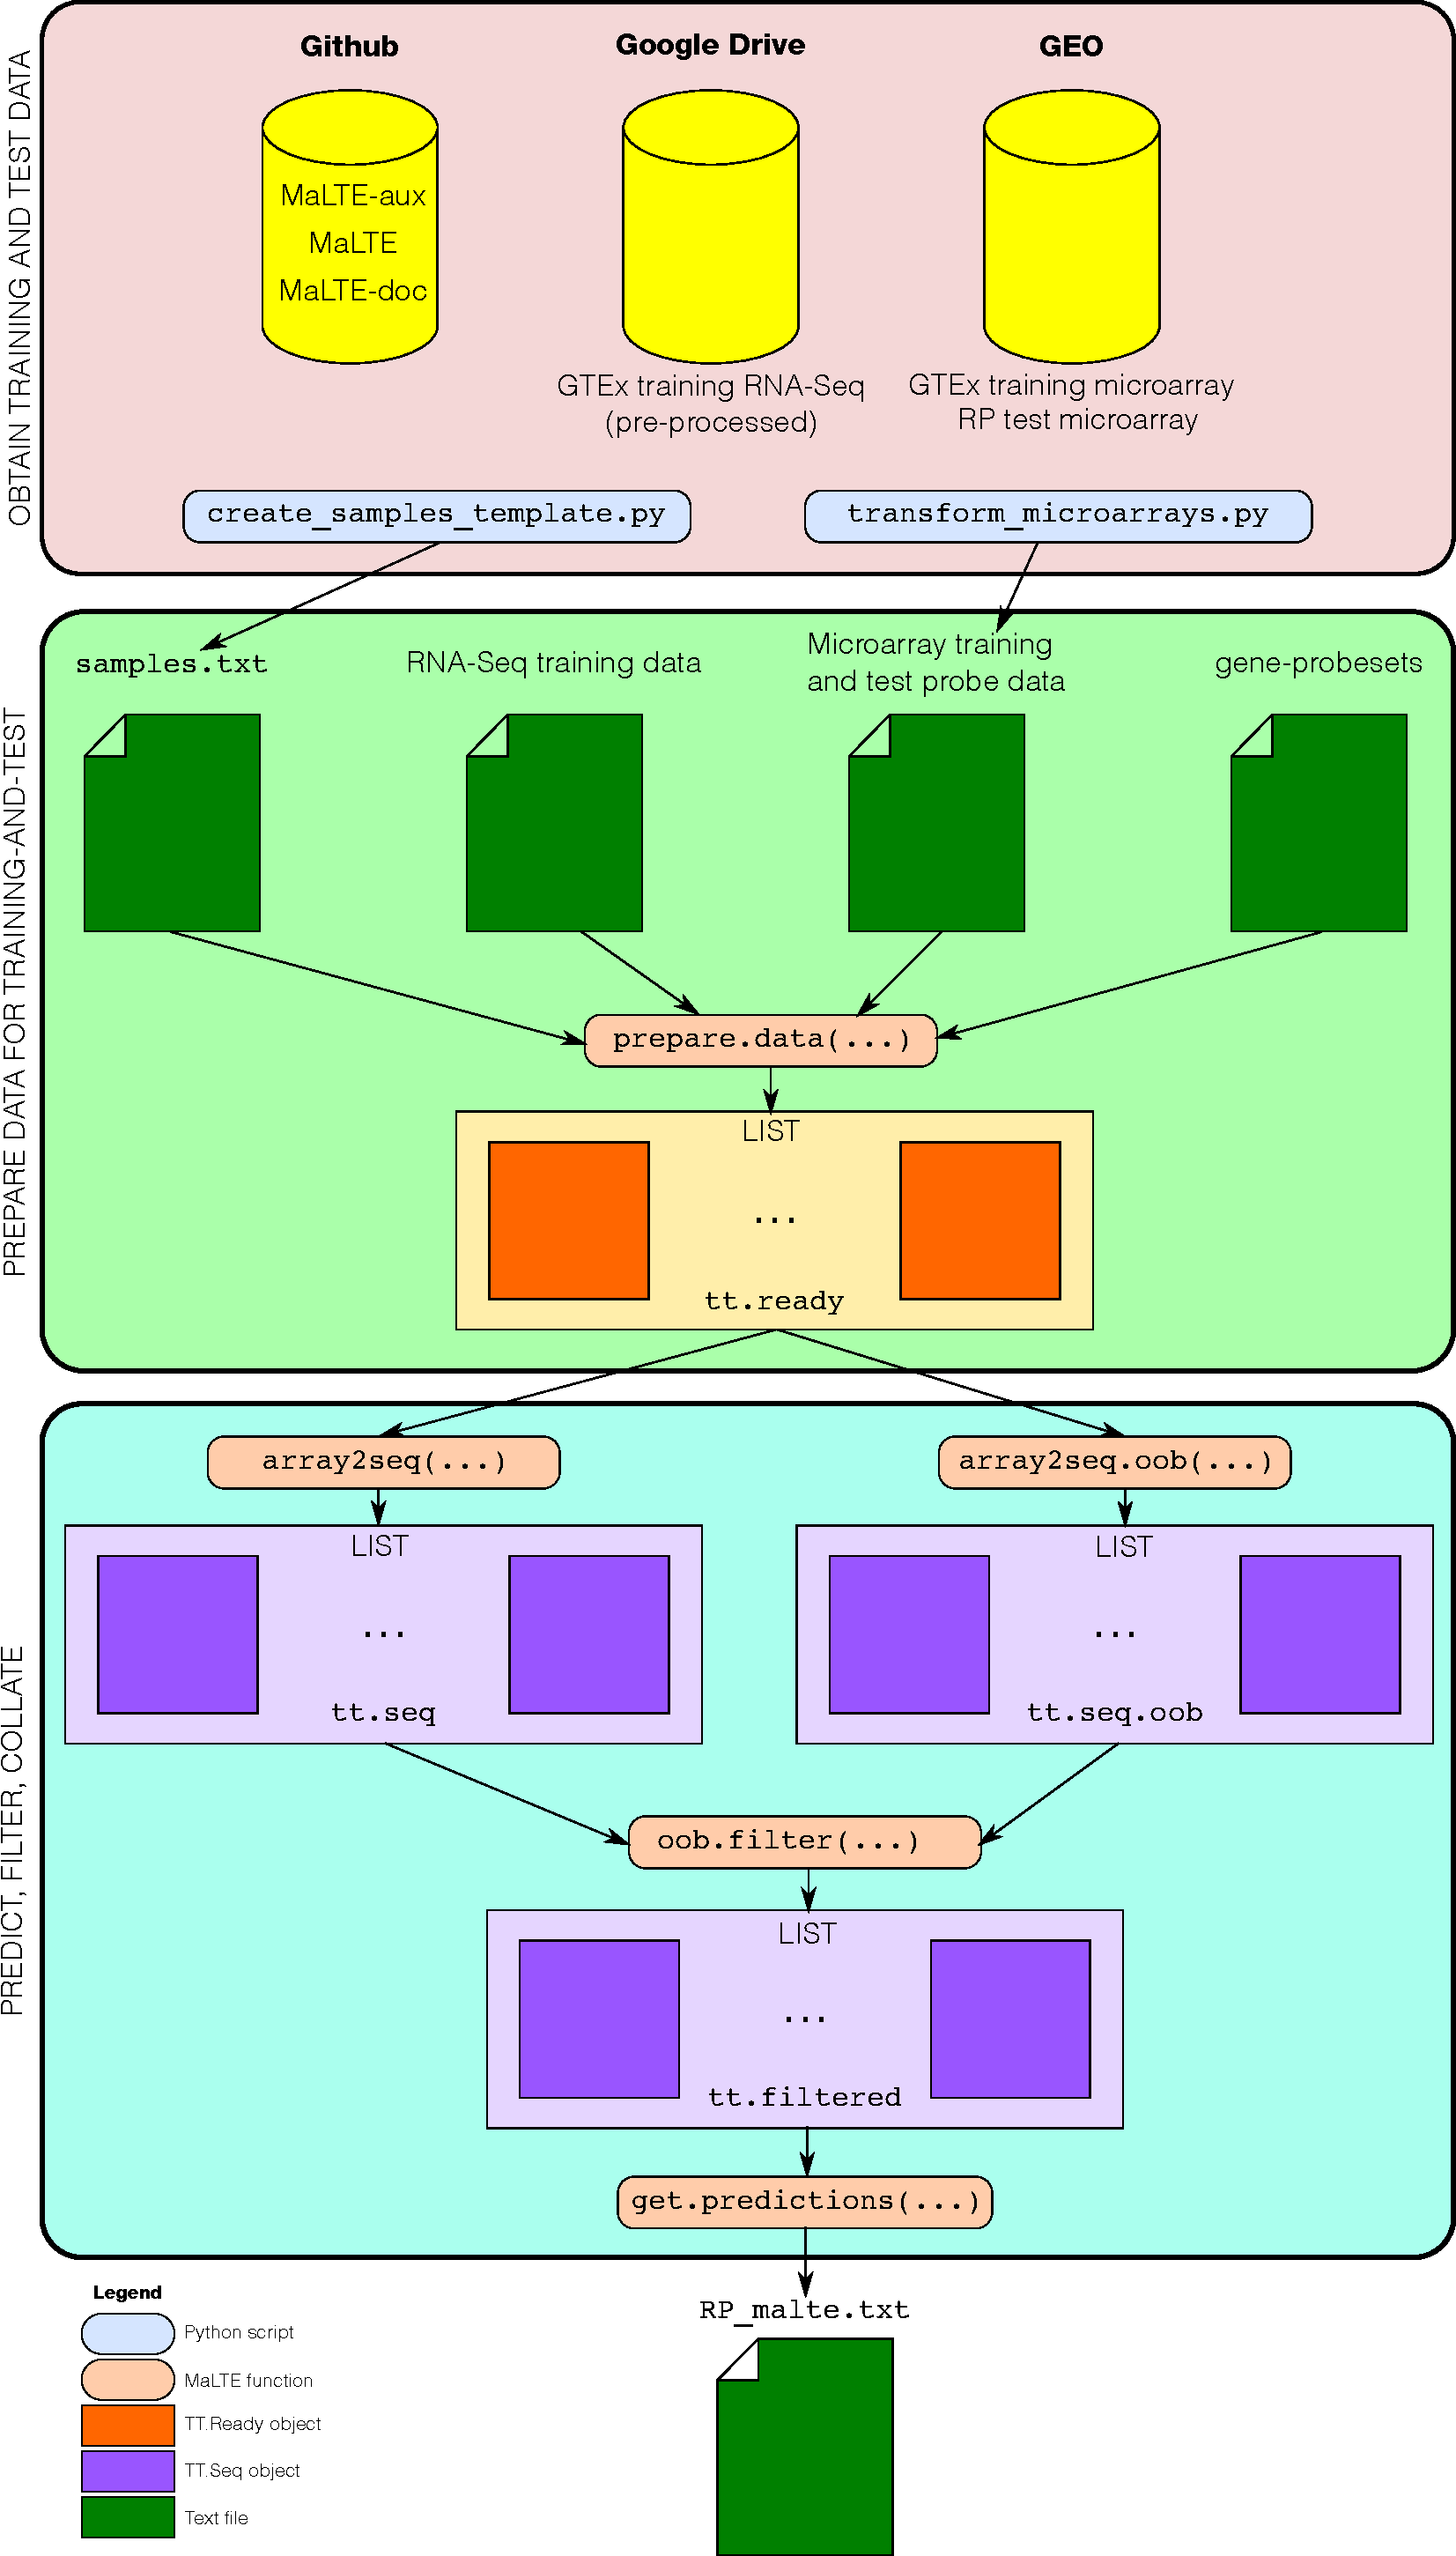
\includegraphics[height=21cm]{schematic1.pdf}
\caption{\textbf{Schematic representing a \textsf{MaLTE} use-case.} The four text files (dark green) are the main input to \textsf{MaLTE}. These files are obtained by processing the training data using the auxiliary scripts.}
\label{fig:usecase}
\end{figure}

In the first step, the user needs to download a set of auxiliary data and scripts before installing the \textsf{MaLTE} \textsf{R} package. The training (and test) data may then be downloaded after which several preprocessing steps may be carried out depending on the type of array involved. For example, we will need to transform the exon array to a gene array. The transformed array data is then quantile normalized to reduce batch effects.

The second and third steps are relatively straightforward and employ only \textsf{MaLTE} functions as outlined in Sections~\ref{gep}.

\subsection{Obtaining Auxiliary Data and Scripts}
\label{usecase:obtaining}

The use-case presented here requires several auxiliary data and scripts to convert the exon array to a gene array. These are all contained in the \textsf{MaLTE-aux} Github repository which may be directly downloaded from \url{https://github.com/polarise/MaLTE-aux}. Click the `Download' button  to get the whole directory as a zip file.

\begin{verbatim}
unzip MaLTE-aux-master.zip
cd MaLTE-aux
\end{verbatim}

Alternatively, it is much faster to use \textsf{git} as follows: 

\begin{verbatim}
git clone git@github.com:polarise/MaLTE-aux.git
cd MaLTE-aux
\end{verbatim}

This directory contains pre-compiled resource files described in Table~\ref{tab:malte_aux}. \textbf{We strongly recommend that all analysis be carried out in this directory.}

\begin{table}
\centering
\begin{tabular}{|l|p{6cm}|}
\hline
\textbf{File} & \textbf{Purpose} \\
\hline
\textit{create\_samples\_template.py} & \multirow{2}{*}{\parbox{6cm}{These script and input data files are used to generate \textit{samples.txt}.}} \\
\textit{training\_samples.txt} & \\
\hline
\textit{transform\_microarrays.py} & \multirow{6}{*}{\parbox{6cm}{The \textsf{Python} script is used to transform the exon array to a gene array. Some probes are omitted in the process. The \texttt{.help} file gives the explicit use of the data files below.}} \\
\textit{transform\_microarrays.help} & \\
 & \\
 & \\
 & \\
 & \\
\hline

\textit{HuEx-1\_0-st-v2.r2.dt1.hg18.full.mps.gz} & \multirow{5}{*}{\parbox{6cm}{Data files required by \textit{transform\_microarrays.py}}} \\
\textit{HuEx-1\_0-st-v2.r2.pgf.txt.gz} & \\
\textit{HuExVsHuGene\_BestMatch.txt.gz} & \\
\textit{HuGene-1\_1-st-v1.r4.mps.gz} & \\
\textit{HuGene-1\_1-st-v1.r4.pgf.txt.gz} & \\
\hline
\textit{gene\_probesets\_HuGene\_Ens72.txt.gz} & \multirow{3}{*}{\parbox{6cm}{Input data files required to run the \textsf{MaLTE} function \texttt{prepare.data()}}} \\ \textit{transcript\_probesets\_HuGene\_Ens72.txt.gz} & \\
 & \\
\hline
\end{tabular}
\caption{Contents of \textsf{MaLTE-aux} and the functions they provide}
\label{tab:malte_aux}
\end{table}

The script \textit{create\_samples\_template.py} compiles the resource file \textit{samples.txt} by choosing a random subset of samples (the user specifies the number) to be used for training specified in \textit{training\_samples.txt}. More information on how it works can be obtained by running 

\begin{verbatim}
./create_samples_template.py --help
\end{verbatim}

The script \textit{transform\_microarrays.py} converts one array to another using several resource files provided in \textsf{MaLTE-aux}. A detailed specification of how to use this script is available in the file \textit{transform\_microarrays.help}.

\subsection{Working Directory Structure}
\label{usecase:directory}

As all analysis will be carried out in \textsf{MaLTE-aux} directory, we need to create two directories for the training and test array CEL files. 

\begin{verbatim}
mkdir GTEx_CEL
mkdir RP_CEL
\end{verbatim}

\subsection{Obtaining MaLTE}
\label{usecase:malte}

\textsf{MaLTE} may be downloaded as a pre-built or source package. Pre-built versions can be found at \url{https://github.com/polarise/MaLTE-packages}. The latest version should be downloaded (files are not sorted by version), ensuring that all prerequisites (see Section~\ref{system}) are installed before installing \textsf{MaLTE}.

\begin{verbatim}
R CMD INSTALL MaLTE_<version>.tar.gz
\end{verbatim} 

The source package requires an installation of \textsf{git} and is obtained as followed:
\begin{verbatim}
git clone git@github.com:polarise/MaLTE.git
\end{verbatim} 

then built with
\begin{verbatim}
R CMD build MaLTE
\end{verbatim}

and installed using \texttt{R CMD INSTALL} as shown above. 

\subsubsection{Creating the file \textit{samples.txt}}
\label{usecase:samples.txt}

The \textit{samples.txt} file is created by running

\begin{verbatim}
./create_samples_template.py
\end{verbatim} 

The names of the test samples should be appended at the bottom of this file using a text editor. For example, to add a test sample called \textit{Test01.CEL} add the following line to \textit{samples.txt}:

\begin{verbatim}
*NA<tab>Test01.CEL
\end{verbatim}

The asterisk (\texttt{`*'}) marks this sample as a test sample and \texttt{`NA'} indicates that RNA-Seq data is not available. Repeat this for as many samples as are present in the test data.

\subsubsection{Obtaining the training data}
\label{usecase:training}

\textbf{\textit{GTEx RNA-Seq data.}} Gene expression levels estimated from RNA-Seq data may be downloaded from \url{http://www.broadinstitute.org/gtex}. The downloaded data needs to be processed to arrive at the training state by excluding extraneous information and converting gene annotation to Ensembl (from GENCODE) then quantile-normalizing only those genes with probe sets. Pre-processed data may be downloaded from \url{https://drive.google.com/file/d/0BxLgaMV5aZahVDNjM29WeGh2NHM/edit?usp=sharing}.

\noindent\\
\textbf{\textit{GTEx gene array data.}} CEL files for the GTEx microarray data are available as a single zipped archive which may be downloaded from GEO archive GSE45878 into the directory \texttt{GTEx\_CEL}. Background-corrected probes should be extracted as follows using the Affymetrix Power Tools function \texttt{apt-cel-extract}, which depends on the Affymetrix GeneChip$^{\text{\textregistered}}$ Human Gene 1.1 ST Array library files available at \url{http://www.affymetrix.com/estore/catalog/prod350003/AFFY/Human-Gene-ST-Array-Strips#1_3}. Select the `Technical Documentation' tab to get a link to the library files.

\begin{verbatim}
apt-cel-extract -o GTEx_probe_intensities.txt \
-c /path/to/HuGene-1_1-st-v1.r4.clf \
-p /path/to/HuGene-1_1-st-v1.r4.pgf \
-b /path/to/HuGene-1_1-st-v1.r4.bgp \
-a pm-gcbg GTEx_CEL/*.CEL
\end{verbatim}

It may be necessary to extract background probes file using \texttt{apt-dump-pgf}.

\begin{verbatim}
apt-dump-pgf \
-p /path/to/HuGene-1_1-st-v1.r4.pgf \
-c /path/to/HuGene-1_1-st-v1.r4.clf \
--probeset-type antigenomic \
-o HuGene-1_1-st-v1.r4.bgp
\end{verbatim}

\noindent\\
\textbf{\textit{Exon array data.}} We outline this procedure using a previously uploaded dataset available under GEO accession GSE43134 into the directory \texttt{RP\_CEL}. The Affymetrix GeneChip$^{\text{\textregistered}}$ Human Exon 1.0 ST Array library files are available from \url{http://www.affymetrix.com/estore/catalog/131452/AFFY/Human-Exon-ST-Array}. Similarly, background-corrected probe fluorescence intensities should be extracted as follows:

\begin{verbatim}
apt-cel-extract \
-o RP_probe_intensities.txt \
-c /path/to/HuEx-1_0-st-v2.r2.clf \
-p /path/to/HuEx-1_0-st-v2.r2.pgf \
-b /path/to/HuEx-1_0-st-v2.r2.antigenomic.bgp \
-a pm-gcbg RP_CEL/*.CEL
\end{verbatim}

\subsection{Transforming exon array probes to gene array probes}
\label{usecase:transforming}

We now run \textit{transform\_microarrays.py} using the following template

\begin{verbatim}
./transform_microarrays.py \
-e RP_probe_intensities.txt \
-g GTEx_probe_intensities.txt \
-c HuExVsHuGene_BestMatch.txt.gz \
-i HuGene-1_1-st-v1.r4.pgf.txt.gz \
-f HuEx-1_0-st-v2.r2.pgf.txt.gz \
-p HuEx-1_0-st-v2.r2.dt1.hg18.full.mps.gz \
-q HuGene-1_1-st-v1.r4.mps.gz \
--huex-out BestMatch_HuEx_probe_intensities.txt.gz \
--huge-out BestMatch_HuGe_probe_intensities.txt.gz
\end{verbatim}

Once the modified probe intensity files have been created they need to be quantile-normalized together with the training data as follows:

\begin{verbatim}
> library( limma )

> # BESTMATCH DATA
> huex.best <- read.table( "BestMatch_HuEx_probe_intensities.txt.gz", 
  header=TRUE,  stringsAsFactors=FALSE,  check.names=FALSE)

> huge.best <- read.table( "BestMatch_HuGe_probe_intensities.txt.gz", 
  header=TRUE,  stringsAsFactors=FALSE,  check.names=FALSE)

> # all raw data
> data <- cbind( huge.best[,8:ncol( huge.best )], 
  huex.best[,8:ncol( huex.best )] )

> # quantile normalisation only
> qnorm.data <- normalizeQuantiles( data, ties=FALSE )
> # save the quantile-normalised data for later 
> # (extracting principal components)
> save( qnorm.data, file="qnorm.data.Rdata" )

> # re-insert probe metadata
> hugeex.qnorm.data <- cbind( huge.best[,1:7], qnorm.data )

> # save to file
> write.table( hugeex.qnorm.data, 
  file="BestMatch_GTEx_RP_probe_intensities_QN.txt", col.names=TRUE, 
  row.names=FALSE,  quote=FALSE,  sep="\t" )
\end{verbatim}

All training data needed is now available to use \textsf{MaLTE}.

\subsection{Preparing the data for training-and-testing}
\label{usecase:preparing}

We can now use \textsf{MaLTE} to prepare the data for training and testing. First, we load the package after launching \textsf{R}.

\begin{verbatim}
> library( MaLTE )
\end{verbatim}

We use the \texttt{prepare.data()} function which takes as arguments the \textit{samples.txt,\\ GTEx\_subset\_gene\_rpkm\_QN.txt, BestMatch\_GTEx\_RP\_probe\_intensities\_QN.txt.gz}, and\\ \textit{gene\_probesets\_HuGene\_Ens72.txt.gz} (available in \textsf{MaLTE-aux} directory).

\begin{verbatim}
> prepare.data( samples.fn=`samples.txt', 
  hts.fn=`GTEx_subset_gene_rpkm_QN.txt.gz’,
  ma.fn=`BestMatch_GTEx_RP_probe_intensities_QN.txt’,
  g2p.fn=`gene_probesets_HuGene_Ens72.txt.gz', raw=TRUE )
\end{verbatim}

We then read in the training and test data.

\begin{verbatim}
> tt.ready = read.data( train.fn=`train_data.tar.gz', 
  test.fn=`test_data.tar.gz' )
\end{verbatim}

\subsection{Prediction}
\label{usecase:prediction}

Prediction can either be performed on the test data training data (out-of-bag, OOB). We outline OOB shortly. First, we need to define training-and-test parameters (additional parameters are specified in Section~\ref{params}).
	
\begin{verbatim}
> tt.params = TT.Params()	# default parameters
\end{verbatim} 

This sets the following values:

\begin{verbatim}
> tt.params
mtry             = 2 
ntree            = 1000 
feature.select   = TRUE 
min.probes       = 15 
cor.thresh       = 0 
OOB              = FALSE 
QuantReg         = FALSE 
Tune (OOB cor.P) = NA
\end{verbatim}

Predictions are performed using the \texttt{array2seq()} function.

\begin{verbatim}
> tt.seq = array2seq( tt.ready, tt.params )
\end{verbatim}

OOB predictions are performed using the \texttt{array2seq.oob()} function.

\begin{verbatim}
> tt.seq.oob = array2seq.oob( tt.ready, tt.params )
\end{verbatim} 

\subsection{Filtering by OOB}
\label{usecase:filtering}

OOB filtering is performed using the \texttt{oob.filter()} function, which takes a \texttt{tt.seq} pair (\texttt{tt.seq} and \texttt{tt.seq.oob}) and a filtering threshold together with the correlation to use for filtering (Pearson (default) or Spearman),
	
\begin{verbatim}
> tt.filtered = oob.filter( tt.seq, tt.seq.oob, thresh=0.5, method=`spearman' )
\end{verbatim}

\subsection{Collating predicted gene expression values}
\label{usecase:collating}

Predicted values should be collated as a data frame using the \texttt{get.predictions()} function. First, we get the names of test samples using the \texttt{get.names()} or \texttt{get.test()} functions.

\begin{verbatim}
> test.names = get.names( samples.fn=`samples.txt', test=TRUE )
> test.names = get.test( samples.fn=`samples.txt' )
\end{verbatim}

The predictions can be quantile-normalized but this may be omitted.
	
\begin{verbatim}
> df.malte.qn = get.predictions( tt.filtered, sample.names=test.names, 
  qnorm=TRUE )
\end{verbatim}

then saved to file

\begin{verbatim}
> write.table( df.malte, file=`RP_malte_OOB_0p5_QN.txt', 
  col.name=TRUE, row.names=FALSE, quote=FALSE, sep=`\t' )
\end{verbatim}

\pagebreak
\section{Experimental features}
\label{experimental}

\subsection{Per-gene/transcript tuning}
\label{experimental:tuning}

Set \texttt{tune.cor.P=TRUE} in \texttt{TT.Params()}

\begin{verbatim}
> tt.params = TT.Params( tune.cor.P=TRUE )
\end{verbatim}

\subsection{Incorporating principal components}
\label{experimental:princomp}

Principal components of probe intensities may be incorporated into the prediction. The same principal component will be used for all genes/transcript therefore they must be incorporated into the \textit{samples.txt} file to be dispatched to all genes/transcripts. We have experimented with the first 10 principal components. 

\begin{verbatim}
> load( "dnorm.data.Rdata" )	# load ‘qnorm.data’ from before
> pc.data = princomp( qnorm.data )

# save the first 10 principal components
> pcs = pc.data$loadings[,1:10]
> samples = read.table( ‘samples.txt', header=TRUE )

# create new samples data frame augmented with principal components
> samples.aug = cbind( samples, pcs )
> colnames( samples.aug ) = paste( ‘P', 1:10, sep=`' )

# create a new samples file
> write.table( samples.aug, file=`samples_aug.txt', 
  col.names=TRUE, row.names=FALSE, quote=FALSE, sep=`\t' )
\end{verbatim}

We then run \texttt{prepare.data()} using \textit{samples\_aug.txt} (instead of \textit{samples.txt} as before) setting the variable \texttt{PCs=TRUE}. This creates two files: \textit{train\_PCs.txt} having the training principal components and a corresponding \textit{test\_PCs.txt}.

\begin{verbatim}
> prepare.data( samples.fn=samples.fn, hts.fn=hts.fn, ma.fn=ma.fn, 
  g2p.fn=g2p.fn, PCs=TRUE )
\end{verbatim} 

Also, we need to run \texttt{read.data()} setting \texttt{PCs.present=TRUE},\\ \texttt{train.PCs.fn=`train\_PCs.txt'} and \texttt{test.PCs.fn=`test\_PCs.txt'}.

\begin{verbatim}
> tt.ready.pc <- read.data( train.fn="train_data.txt.gz", 
  test.fn="test_data.txt.gz", PCs.present=TRUE, 
  train.PCs.fn="train_PCs.txt", test.PCs.fn="test_PCs.txt"  )
\end{verbatim} 

The principal components are now embedded in the data for each gene.

% \pagebreak
% \section{License}
% \label{license}
% \begin{verbatim}
% Copyright (C) 2013  Paul K. Korir 
% 
% This program is free software: you can redistribute it and/or modify it
% under the terms of the GNU General Public License as published by the 
% Free Software Foundation, either version 3 of the License, or (at your
% option) any later version.
% 
% This program is distributed in the hope that it will be useful, but 
% WITHOUT ANY WARRANTY; without even the implied warranty of MERCHANTABILITY
% or FITNESS FOR A PARTICULAR PURPOSE.  See the GNU General Public License 
% for more details.
% 
% You should have received a copy of the GNU General Public License along 
% with this program.  If not, see <http://www.gnu.org/licenses/>.
% \end{verbatim}

\end{document}
